\section{Analysis and geometry: which solution does training find?}
\label{sec:analysis}

\subsection{Why trained networks generalize: singular learning theory}

A trained network is a setting of parameters chosen to fit its \emph{training data}---the finite set of examples it was optimized on. The trouble is that a large network has astronomically many settings that fit those examples perfectly, and they disagree wildly everywhere else; the optimizer---\glsfirst{gradient-descent}{gradient descent}, which repeatedly nudges the parameters downhill on the training error---must land on one of them. For safety, the selected solution matters: a network that behaved well while we were watching may behave differently once deployed. So why do the solutions found by training \emph{generalize}---predict well on fresh data from the same source---when so many other data-fitting solutions would not? These networks reach zero error even when the labels are replaced by pure noise, and a two-layer network with only $2n+d$ parameters can fit \emph{any} labeling of $n$ points in $\mathbb{R}^d$ (Zhang et al.~\cite{zhang2017}); the classical bounds that explain generalization by counting parameters say nothing here.

A different and more general answer comes from \emph{singular learning theory}~\cite{watanabe2009}. Realistic models are \emph{singular}: distinct parameters compute the same function, typically in continuous families, so the optimal set is not an isolated point but a positive-dimensional variety---itself typically singular---flat to second order along its own directions (Figure~\ref{fig:singular-geometry}). The classical large-sample asymptotics all assume an isolated, curved optimum; the right replacements come from algebraic geometry. One caveat: the theory is exact for \emph{Bayesian} learning, not directly for stochastic gradient descent (gradient descent driven by noisy, small-batch estimates of the gradient)---bridging the two is the problem \emph{Opposing staircases} below. The two are closer than they appear: Khan and Rue~\cite{khan2023} derive stochastic gradient descent, along with many other optimizers, as approximations of a single Bayesian update rule.

\begin{figure}[ht]
\centering
\begin{tikzpicture}[>=Stealth, x=1cm, y=1cm]
  \begin{scope}
    \node[font=\small] at (0,1.75) {regular optimum};
    \draw[->, gray!70] (-1.5,-1.25) -- (1.7,-1.25) node[right, font=\scriptsize] {$w_1$};
    \draw[->, gray!70] (-1.5,-1.25) -- (-1.5,1.35) node[above, font=\scriptsize] {$w_2$};
    \foreach \r in {0.35,0.65,0.95,1.25} {
      \draw[gray!55] (0,0) ellipse ({1.15*\r} and {0.55*\r});
    }
    \fill[blue!60!black] (0,0) circle (1.4pt) node[above right, font=\scriptsize] {$w_0$};
    \node[font=\scriptsize, align=center] at (0,-1.65) {isolated quadratic bowl\\penalty $d/2$};
  \end{scope}
  \begin{scope}[xshift=5.2cm]
    \node[font=\small] at (0,1.75) {singular optimum};
    \draw[->, gray!70] (-1.5,-1.25) -- (1.7,-1.25) node[right, font=\scriptsize] {$w_1$};
    \draw[->, gray!70] (-1.5,-1.25) -- (-1.5,1.35) node[above, font=\scriptsize] {$w_2$};
    \draw[very thick, blue!60!black] (-1.05,-0.12) .. controls (-0.55,0.35) and (0.45,-0.35) .. (1.05,0.12);
    \foreach \s in {0.25,0.5,0.75,1.0} {
      \draw[gray!55] (-1.05,-0.12-\s/2) .. controls (-0.55,0.35-\s) and (0.45,-0.35-\s) .. (1.05,0.12-\s/2);
      \draw[gray!55] (-1.05,-0.12+\s/2) .. controls (-0.55,0.35+\s) and (0.45,-0.35+\s) .. (1.05,0.12+\s/2);
    }
    \fill[blue!60!black] (-0.0375,0) circle (1.4pt)
      node[above, font=\scriptsize, fill=white, inner sep=0.5pt] {$w_0$};
    \node[right, font=\scriptsize, blue!60!black] at (1.05,0.12) {$W_0$};
    \node[font=\scriptsize, align=center] at (0,-1.65) {curve of equivalent optima\\penalty $\lambda=\tfrac12<\tfrac d2$};
  \end{scope}
\end{tikzpicture}
\caption{Regular asymptotics treat the optimum as an isolated quadratic bowl, giving the classical $\tfrac d2\log n$ complexity penalty. Singular learning theory allows a whole variety of parameters to compute the same function: in the right panel the optimal set is a curve $W_0$ through $w_0$, and the penalty $\lambda=\tfrac12$ is strictly smaller than $\tfrac d2=1$, as it is whenever the optimal set has positive dimension.}
\label{fig:singular-geometry}
\end{figure}

% Toy singularity added 2026-07-13 (Codex slope report): one computation the reader
% owns before the formal setup; the exponent/log pair previews (lambda, m).
A toy computation shows what singularity buys. Take first the regular loss $K(w)=w^2$ on the line: the set where $K\le\varepsilon$ is an interval of length $2\sqrt\varepsilon$, so the volume of near-optimal parameters scales as $\varepsilon^{1/2}$---the exponent is $d/2$ with $d=1$. Now take $K(a,b)=a^2b^2$ on the square $[-1,1]^2$. Its zero set is not a point but the union of the two axes, crossing at a singularity, and the region where $K\le\varepsilon$ is a neighborhood of the axes of area of order $\varepsilon^{1/2}\log(1/\varepsilon)$: the exponent stays $1/2$ rather than rising to $d/2=1$, and a logarithm appears. A singular loss has far more near-optimal parameters than its dimension suggests, and the pair (exponent, power of the logarithm) is the simplest instance of the learning coefficient and multiplicity about to be defined.

To make this precise, fix a model $p(x\mid w)$ with parameter $w$ in a compact $W\subseteq\mathbb{R}^d$, a prior $\varphi$ on $W$ (a probability density encoding which parameters are plausible before any data is seen), and a true distribution $q_0(x)=p(x\mid w_0)$ lying in the model. (The subscript keeps the truth $q_0$ apart from the belief $q$ of Section~\ref{sec:epistemics}.) Write
\[
   K(w)=\mathrm{KL}\!\bigl(q_0 \,\big\|\, p(\cdot\mid w)\bigr)=\int q_0(x)\log\frac{q_0(x)}{p(x\mid w)}\,dx ,
\]
the Kullback--Leibler divergence of Section~\ref{sec:epistemics}, so that the set of \emph{true parameters} $W_0=K^{-1}(0)$ is exactly where the model recovers $q_0$.

Given $n$ i.i.d.\ samples $X_1,\dots,X_n$, the central object is the \emph{Bayes free energy}---equivalently the negative log marginal likelihood, the codelength the model assigns to the data,
\[
   \bar F_n \;=\; -\log \int_W \prod_{i=1}^n p(X_i\mid w)\,\varphi(w)\,dw .
\]
(The bar is part of the name; $\bar F_n$ is the random free energy of the sample, not an expectation.) Normalizing the same integrand gives the \emph{posterior} $\propto\prod_i p(X_i\mid w)\,\varphi(w)$---the prior reweighted by how well each parameter fits the data---so $\bar F_n$ is minus the log of its normalizer. This free energy is not the variational free energy $F(q,x)$ of Section~\ref{sec:epistemics}: that one scores a belief against a single observation, this one scores the whole model against a whole sample. The shared name reflects a shared shape, minus the log of a normalizing integral.

Take first the \emph{regular} case: the model is \emph{identifiable} (distinct parameters give distinct distributions) and the optimal set is a single point $W_0=\{w_0\}$ at which the Hessian of $K$---the \emph{Fisher information} $I(w_0)$---is positive-definite. Then the integrand defining $\bar F_n$ concentrates in a shrinking neighborhood of $w_0$; expanding $\log p(X_i\mid w)$ to second order there makes the integral Gaussian, contributing a volume factor $(2\pi/n)^{d/2}\det I(w_0)^{-1/2}$. Taking $-\log$,
\[
   \bar F_n \;=\; nS_n \;+\; \tfrac{d}{2}\log n \;+\; O_p(1),
   \qquad S_n=-\tfrac1n\textstyle\sum_i\log q_0(X_i),
\]
where $S_n$ is the empirical entropy and the remainder is bounded in probability.\footnote{$O_p(1)$ means \emph{bounded in probability}: for every $\varepsilon>0$ there is an $M$ with $\Pr(|\,\cdot\,|>M)<\varepsilon$ for all large $n$.} The complexity penalty is exactly half the parameter count. Watanabe's theorem is the singular replacement, in which $d/2$ gives way to an invariant of the singular geometry.

\begin{theorem*}[Watanabe's free-energy asymptotics~\cite{watanabe2009}]
For a singular model satisfying Watanabe's regularity conditions (real-analyticity and a mild variance bound\footnote{The \emph{relatively finite variance} condition: writing $f(x,w)=\log(q_0(x)/p(x\mid w))$, $K(w)=\mathbb{E}_{q_0} f(X,w)$, and $V(w)=\mathbb{E}_{q_0} f(X,w)^2$, one assumes $V(w)\le C\,K(w)$ near the optimal set---the variance of the log-likelihood ratio is controlled by its mean.}), as $n\to\infty$,
\begin{equation}\label{eq:free-energy}
   \bar F_n \;=\; n\,S_n \;+\; \lambda\log n \;-\; (m-1)\log\log n \;+\; O_p(1),
\end{equation}
where the \emph{learning coefficient} $\lambda>0$---the \emph{real log canonical threshold} (\textup{\textsc{rlct}}) of $K$ relative to the prior $\varphi$---and the integer $m\in\{1,\dots,d\}$, its \emph{multiplicity}, take the places of the $d/2$ and the $1$ of the regular case. The $O_p(1)$ remainder converges in distribution.\footnote{In the regular case the limit is $C-\tfrac12\chi^2_d$ for a constant $C$---the Bayesian shadow of Wilks' theorem, since the log-likelihood-ratio statistic $2\bigl(\sup_w\textstyle\sum_i\log p(X_i\mid w)-\sum_i\log p(X_i\mid w_0)\bigr)\Rightarrow\chi^2_d$. In a singular model the limit is in general non-Gaussian, a functional of a Gaussian process on the manifold obtained by resolving the singularities of $K$.} The same coefficient controls generalization: writing $\hat p_n$ for the posterior average of $p(\cdot\mid w)$, the \emph{generalization error} $G_n=\mathrm{KL}(q_0\,\|\,\hat p_n)$ obeys $\mathbb{E}[G_n]=\lambda/n+o(1/n)$.
\end{theorem*}

The meaning of $\lambda$ is volume growth: the prior volume of the set $\{w\in W : K(w)\le\varepsilon\}$ of parameters fitting the truth to within $\varepsilon$ scales like $\varepsilon^{\lambda}$ times $(\log(1/\varepsilon))^{m-1}$, so smaller $\lambda$ means near-optimal parameters are more plentiful. To compute $\lambda$ for a given model, one resolves the singularities of $K$ (Hironaka~\cite{hironaka1964}).

In the regular case, $\lambda=d/2$ and $m=1$, and the theorem recovers the regular asymptotic expansion above; in a singular model $\lambda\le d/2$, often strictly. The comparison localizes: restrict the integral defining $\bar F_n$ to a neighborhood of one true parameter, and the expansion \eqref{eq:free-energy} holds with that neighborhood's own coefficient. Among the true parameters---all fitting the truth exactly, all weighted by the prior---the posterior share of the most degenerate neighborhoods, those of smallest local $\lambda$, grows with $n$. In this Bayesian setting the posterior concentrates, on its own, on the solutions that the formula $\mathbb{E}[G_n]=\lambda/n$ marks as best-generalizing. This is the theory's rendering of the slogan that learning prefers ``simpler'' solutions: simplicity means a more degenerate geometry, not fewer parameters.

The degeneracy behind a small $\lambda$ is largely \emph{structural}: it comes from directions in parameter space along which the function does not change---for instance those freed when an internal unit is effectively switched off---and these are what pull $\lambda$ below $d/2$. The symmetries are not a defect to be engineered away: within the theory, it is the degeneracy that pulls the generalization error $\lambda/n$ below the classical rate $d/(2n)$.

The coefficient $\lambda$ need not be found by hand. Introduce a knob $\beta>0$, an \emph{inverse temperature}, and the \emph{tempered posterior}
\[
   p_\beta(w)\;\propto\;\varphi(w)\,e^{-\beta n L_n(w)},
   \qquad L_n(w)=-\tfrac1n\textstyle\sum_i\log p(X_i\mid w),
\]
which interpolates between the prior ($\beta=0$) and concentration on the best-fitting parameters ($\beta\to\infty$). (In statistics, taking $\beta<1$ hedges against a misspecified model: Gr\"unwald's ``Safe Bayesian'' learns $\beta$ from the data~\cite{grunwald2012}, and Alquier and Ridgway prove that tempered posteriors still concentrate~\cite{alquier2020}.) At inverse temperature $\beta=1/\log n$, the average of $nL_n$ over the tempered posterior exceeds its minimum by $\lambda\log n$, to leading order~\cite{watanabe2013}. So $\lambda$ can be \emph{estimated} by sampling the tempered posterior, needing neither the true distribution nor an explicit resolution of singularities. That practicality is what lets the theory meet networks far too large to analyze by hand.

What one estimates is not the global $\lambda$ but the \emph{local learning coefficient}: the same invariant computed in a neighborhood of the particular solution $w^\star$ that training actually reached, measuring how degenerate \emph{that} solution is~\cite{lau2023}. As a network trains, its local learning coefficient jumps at discrete moments---\emph{phase transitions}, where the solution moves to a qualitatively new, differently-degenerate part of the landscape as a new piece of internal structure forms. Tracking these jumps is the program of \emph{developmental interpretability}: so far on relatively small networks and with preliminary validation, though the same estimators have already surfaced tens of thousands of candidate structures inside a billion-parameter language model~\cite{murfet2026}.

Two networks can fit the training data identically and yet compute by different internal mechanisms, hence behave differently on inputs outside that data---what ordinary testing, which only probes behavior on data, cannot detect. The singular geometry governs \emph{which} mechanism training selects, and the selection need not favor the mechanisms we would prefer: the most degenerate solution---largest in volume, smallest in $\lambda$---may implement the behavior we intended, or a shortcut that mimics it on the training distribution and fails beyond it. Whether geometric degeneracy favors mechanisms that are also interpretable and robust is, for safety, the question this program must answer; the case that alignment turns on such questions is made in~\cite{lehalleur2025}.

\begin{openproblem}[Does geometric simplicity force a legible mechanism?]
Fix an odd integer $p$ and $H\geq 2p-1$. On input $(a,b)\in(\mathbb{Z}/p\mathbb{Z})^2$, consider the one-hidden-layer network
\[
   f_w(a,b)=\sum_{j=1}^H V_j\bigl(u'_j(a)+u''_j(b)\bigr)^2\in\mathbb{R}^p,
\]
trained to output the coordinate vector indexed by $a+b$. The $j$th summand is one hidden neuron: it adds two entries from the lookup tables $u'_j,u''_j\colon\mathbb{Z}/p\mathbb{Z}\to\mathbb{R}$, squares the result, and writes the vector $V_j$ to the output. Fourier inversion gives exact fits in which each neuron that contributes nontrivially carries a single frequency: for some $k$, both lookup tables are a constant plus a linear combination of $\cos(2\pi k\,\cdot/p)$ and $\sin(2\pi k\,\cdot/p)$. Up to a change of basis, this is the algorithm found by reverse-engineering trained networks~\cite{nanda2023}.

Is this Fourier structure forced by singular geometry? In a fixed closed ball containing one of these Fourier fits, prove or refute that every exact fit of smallest local learning coefficient has this single-frequency form, apart from neurons whose contribution vanishes identically. The first non-vacuous case is $p=5$ with nine hidden neurons: use its Fourier symmetries to classify the most singular exact fits, or find a non-Fourier one by computer algebra. A proof would connect geometric simplicity to a mechanism one can read from the weights; a counterexample would show that the two notions of simplicity can part ways.
\end{openproblem}

\subsection{Learning in stages}

Learning does not always proceed smoothly; long flat stretches give way to sudden changes. The modular-addition task above is the best known example: a network fits its training data early but generalizes only much later, and abruptly. This is \emph{grokking}~\cite{nanda2023}.\footnote{Grokking and the staircase below are cousins, not the same phenomenon: grokking is a delayed jump in performance on \emph{held-out} data after the training loss is already low, whereas the staircase is a stepwise fall of the \emph{training} loss itself. Both are read, in this program, as transitions between differently-singular regions of parameter space.}

The simplest solvable model of such stepwise learning is the deep \emph{linear} network: a product of matrix factors $W_L\cdots W_1$ fit to a target linear map by \emph{gradient flow} (gradient descent in continuous time) on squared error. The composite map is linear, but as a function of the separate factors the loss is a non-convex polynomial, so the flow is genuinely nonlinear. Saxe, McClelland, and Ganguli~\cite{saxe2014} show that when the inputs are \emph{whitened} (linearly transformed to have identity covariance), the singular value decomposition of the input--output correlation matrix \emph{decouples} the dynamics into independent scalar equations, one per singular value $s$: each is the logistic ordinary differential equation $\tau\dot a=2a(s-a)$, whose solution rises sigmoidally from near $0$ to $s$ in time of order $\tau/s$ (Figure~\ref{fig:staircase}). The decoupling and the scalar solutions are exact; the initialization then sets the order of events: for comparably small initial coefficients, modes with larger $s$ turn on earlier, and when their turn-on times are well separated the training error falls not smoothly but in a staircase---long plateaus near saddle points of the loss, each broken by a sharp drop as the next mode is acquired. Here ``which structure the network learns, and in what order'' has a closed-form answer.

The staircase survives beyond the linear case: Abbe, Boix-Adser\`a, and Misiakiewicz~\cite{abbe2023} prove that training a two-layer network on a \emph{sparse} target---one depending on only a few of its inputs---again proceeds in stages, saddle to saddle, with the waiting time before each stage set by a combinatorial \emph{leap complexity} measuring how many inputs must be assembled at once. Carrying such exact accounts to the nonlinear networks used in practice is open.

\begin{figure}[ht]
\centering
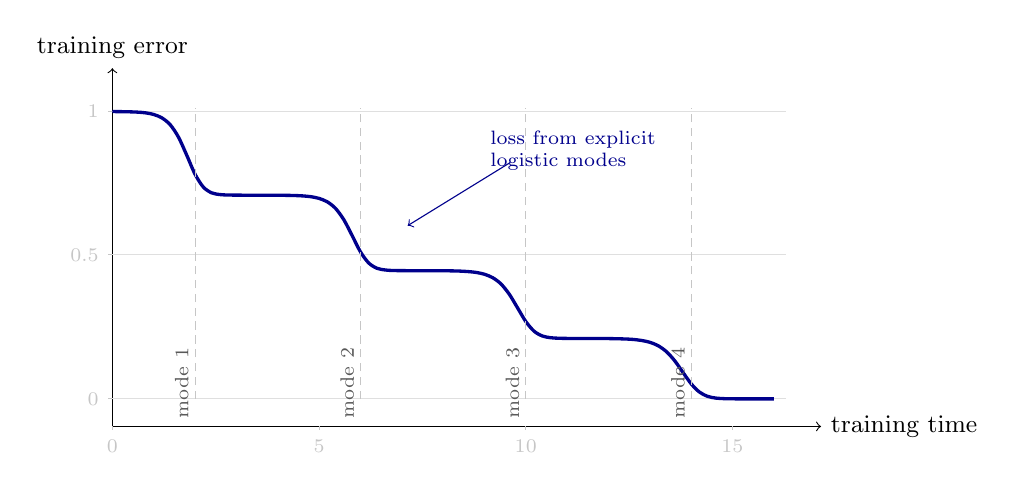
\begin{tikzpicture}[x=1cm,y=1cm]
  \draw[->] (0,0) -- (9,0) node[right] {\small training time};
  \draw[->] (0,0) -- (0,4.55) node[above] {\small training error};
  \foreach \x/\lab in {0/0,2.625/5,5.25/10,7.875/15} {
    \draw[gray!45] (\x,0) -- (\x,-0.05) node[below,font=\scriptsize] {\lab};
  }
  \foreach \y/\lab in {0.35/0,2.18/0.5,4.0/1} {
    \draw[gray!45] (0,\y) -- (-0.05,\y) node[left,font=\scriptsize] {\lab};
  }
  \draw[gray!25] (0,0.35) -- (8.55,0.35);
  \draw[gray!25] (0,2.18) -- (8.55,2.18);
  \draw[gray!25] (0,4.0) -- (8.55,4.0);
  \draw[blue!55!black,very thick,smooth] plot coordinates {
    (0.000,3.999) (0.105,3.998) (0.210,3.996) (0.315,3.992) (0.420,3.983)
    (0.525,3.962) (0.630,3.918) (0.735,3.831) (0.840,3.673) (0.945,3.443)
    (1.050,3.203) (1.155,3.040) (1.260,2.967) (1.365,2.945) (1.470,2.939)
    (1.575,2.938) (1.680,2.937) (1.785,2.937) (1.890,2.937) (1.995,2.937)
    (2.100,2.936) (2.205,2.935) (2.310,2.933) (2.415,2.928) (2.520,2.918)
    (2.625,2.896) (2.730,2.852) (2.835,2.768) (2.940,2.624) (3.045,2.424)
    (3.150,2.218) (3.255,2.076) (3.360,2.009) (3.465,1.987) (3.570,1.980)
    (3.675,1.979) (3.780,1.978) (3.885,1.978) (3.990,1.978) (4.095,1.978)
    (4.200,1.977) (4.305,1.976) (4.410,1.973) (4.515,1.967) (4.620,1.956)
    (4.725,1.933) (4.830,1.889) (4.935,1.810) (5.040,1.680) (5.145,1.507)
    (5.250,1.333) (5.355,1.210) (5.460,1.149) (5.565,1.127) (5.670,1.120)
    (5.775,1.118) (5.880,1.118) (5.985,1.118) (6.090,1.117) (6.195,1.117)
    (6.300,1.116) (6.405,1.114) (6.510,1.111) (6.615,1.105) (6.720,1.092)
    (6.825,1.069) (6.930,1.026) (7.035,0.951) (7.140,0.836) (7.245,0.688)
    (7.350,0.542) (7.455,0.437) (7.560,0.382) (7.665,0.360) (7.770,0.353)
    (7.875,0.351) (7.980,0.350) (8.085,0.350) (8.190,0.350) (8.295,0.350)
    (8.400,0.350)
  };
  \foreach \x/\name in {1.05/1,3.15/2,5.25/3,7.35/4} {
    \draw[gray!45,densely dashed] (\x,0.35) -- (\x,4.05);
    \node[font=\scriptsize,gray!70!black,rotate=90,anchor=south] at (\x+0.04,0.55) {mode \name};
  }
  \node[font=\scriptsize,align=left,blue!55!black] at (5.85,3.5)
    {loss from explicit\\logistic modes};
  \draw[->,blue!55!black] (5.05,3.35) -- (3.75,2.55);
\end{tikzpicture}
\caption{A learning staircase computed from the deep-linear solution of Saxe et al. In mode $i$, $s_i$ is the target singular value and $a_i(t)$ is the coefficient learned by time $t$, satisfying $\tau\dot a_i=2a_i(s_i-a_i)$. The curve plots normalized training error $\sum_i(s_i-a_i(t))^2$ for $\tau=0.5$ and $s=(1,0.95,0.9,0.85)$, with small initial coefficients chosen so the four modes turn on at separated times. Each mode turning on produces one drop.}
\label{fig:staircase}
\end{figure}

\begin{openproblem}[Opposing staircases]
Watanabe's theorem is Bayesian; gradient descent is not. (What bridging the two would mean for safety is discussed in~\cite{lehalleur2025}.) Build the bridge first in the deep-linear staircase above, where both sides are explicit. Each plateau sits at a saddle where only the $k$ largest modes have been learned, and there the definition itself is part of the problem: the local learning coefficient is defined at a local \emph{minimum}, as the volume exponent of the set of nearby parameters fitting almost as well, but a saddle has descent directions, so that volume does not shrink to zero. Formulate the right local invariant at the $k$th saddle (one candidate, the \emph{two-sided} exponent: the volume of nearby parameters whose loss lies within $\varepsilon$ of the saddle's, above or below, shrinks like $\varepsilon^{\lambda}$), compute it for the deep-linear network, and prove or refute the monotone picture that gives this problem its name: as gradient flow descends the staircase of losses, the invariant that controls generalization climbs an opposing staircase. As a first check, the estimator of Lau et al.~\cite{lau2023} runs at any parameter, saddle or not; run it along a simulated staircase and see.
\end{openproblem}

\subsection{Generalization beyond the training distribution}

The theory above concerns generalization \emph{in distribution}: test data drawn from the same law as the training data. The safety-critical regime is the opposite one, \emph{out of distribution}---how a trained system behaves on inputs unlike anything it saw in training---and there the gap between fitting and understanding reopens. Two parameter settings with identical training loss can implement different mechanisms (as above) and therefore extrapolate differently; which extrapolation gradient descent selects is, at present, something we observe after the fact rather than predict.

In \emph{goal misgeneralization}~\cite{langosco2022}, a system under \emph{distribution shift}---a deployment input distribution unlike the one it trained on---keeps its \emph{capabilities} while pursuing a \emph{different goal} from the one intended. The standard example is an agent trained to collect a coin in a video game where the coin always sat at the right end of the level: it learned ``move right,'' not ``reach the coin,'' and the two came apart the moment the coin moved. Capable but misdirected is the dangerous quadrant, and it is invisible to any testing that stays in distribution.

The pattern is old enough to have a name, \emph{Goodhart's law}: a proxy optimized hard enough stops tracking the goal it stood for. On the training levels, ``move right'' was a perfect proxy for ``reach the coin,'' so optimization could not tell them apart; the shift revealed which one the network had learned. Reward hacking (Section~\ref{sec:epistemics}) is the same law during training; goal misgeneralization is the law at deployment.

\begin{openproblem}[A predictive theory of out-of-distribution generalization]
In the coin-collecting environment of Langosco et al.~\cite{langosco2022}, reduced to one dimension, two policies fit the training data perfectly: ``move right'' (the proxy) and ``go to the coin'' (the intended goal), which agree whenever the coin sits at the right end. Train a two-layer network by gradient descent to imitate optimal play, randomizing the coin's position in an $\varepsilon$-fraction of training episodes. Determine the probability, over the random initialization, that the trained network follows the proxy on a probe state where the two policies disagree, as a function of $\varepsilon$, the width, and the input encoding. For linear policies the answer is a theorem---the encoding, not the initialization, decides---and the standard infinite-width limits follow it; for networks of finite width it is open at every $\varepsilon$, including $\varepsilon=0$, already at width two.
\end{openproblem}

% \noindent\emph{Entry points.} Algebraic geometry (resolution of singularities, log canonical thresholds), statistical mechanics, probability, dynamical systems, statistical learning theory.
